\documentclass[../main.tex]{subfiles}

\begin{document}

\subsection{Overwiew}
\begin{figure}[bh]
    \centering
    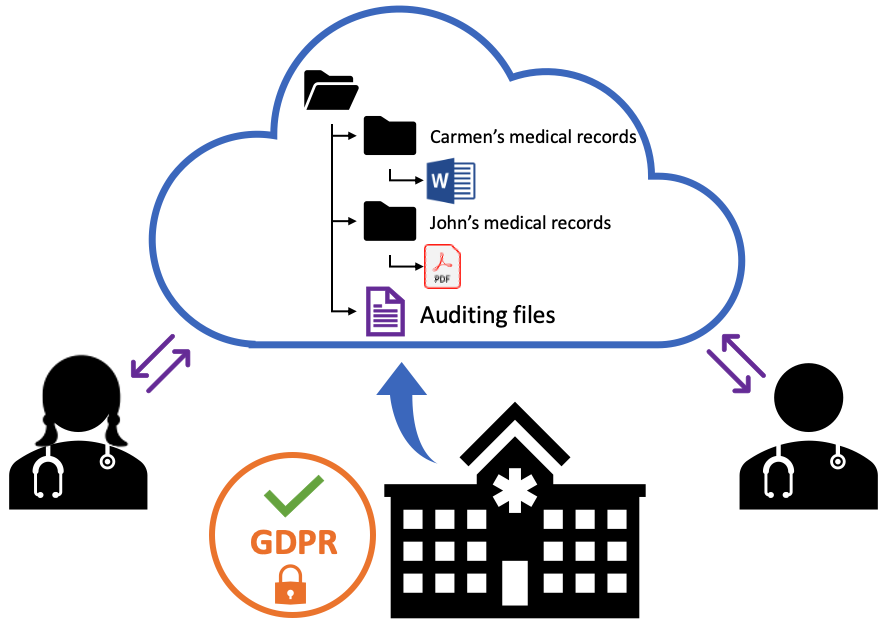
\includegraphics[width=0.75\textwidth]{../images/problem_overview}
    
    \label{problem_description:overview}
    \caption{Representation of the real life situation}
\end{figure}
\par As explained in the introduction, we are in a world were everything is being digitized and uploaded on remote storage. This raises an important question about data privacy: how can I preserve my confidential information, against the Cloud itself, while still being able to harness the power of the Cloud. For example, one of the most notorious power of Cloud Storage is the ability to share part of the storage with other users. \par This situation becomes even more interesting in the healthcare domain. If we look at an hospital, many services must share the medical record of a single patient, as depicted in Figure \ref{problem_description:overview}. How can those parties share this record while still preserving its confidentiality. Even more interesting, once we allow a service to access the record, how can we efficiently revoke their right to read this record ?
\par Along with keeping the data privacy, keeping track of who has accessed or edited a given file is one of the key principles in the new European General Data Protection Regulation (GDPR) established in 2018. This regulations states that: "\textit{All EU institutions have the legal obligation to keep a central register of records of activities processing personal data}". This means that in practice, every time a doctor access the medical record of a patient, he must provides the purpose of this act. Meaning that we need to securely store those information. We also want to be able to retrieve them, in an instant, in case of a GDPR check. Most of all, we must prevent anyone from being able to tamper with those logs, or at least, spot that they have been altered.

\subsection{Design Goals}
\par From reading the previous section, we can deduce the different goals that our solution wishes to reach.
\par \textbf{Practicality}: First of all, we want our solution to be transparent to the doctors. Their typical workflow should not be affected by the transition. This also means that their should not be a consequent overhead while using the new filesystem. We are not considering the complexity of the installation process as it is an orthogonal problem, that a technical professional could handle with ease. However, once the application is up and running, any technical intervention should not longer be required. On top of that, allowing doctors to access a resource about a patient should fast and easy, at the reach of anyone. The revocation process should be equivalently easy and accessible.
\par \textbf{Strong access policy}: The filesystem should also maintain a strong and secure access policy. Only allowed doctors can access the filesystem and even in the filesystem another access policy should be established to protect certain file or directory. The importance of these access policies forces them to be encrypted and tamper evident. In practice, the first step after the installation is to register all the doctors to the filesystem. This is handled by the administrator, he is the only one who has the right to register or revoke a doctor from the filesystem. During this process, the administrator defines who is in charge of giving access to certain part of the filesystem, for example the secretary, we will call this actor the owner. Lastly, the doctor will be able to access a patient data only when the owner allows him to do so. The owner can, if he wants, define a limited time window during which the doctor has access to the data.
\par \textbf{Portability}: No matter the computer the doctor is using, as long as it has been setup, he must be able to access the filesystem with correct access policy. Beforehand, he only needs to prove its identity to the computer. In a real life example, we can consider that the doctor must first scan his badge in order to log in. This procedure could be a realistic identity check, of course, in this scenario, the badge must be provided with some kind of secret in the first place.
\par \textbf{Security}: Any unauthorized entities can't gain any information about the patients, even their name should be kept confidential. Unauthorized entities may include the Cloud Storage, entities trying to spy on the communication, or simply a lambda user that found a way to get his hand on the entirety of the shared folders.
\par \textbf{Write-only auditing files}: Lastly, every action taken by a doctor, may it be reading / editing / removing a file, must be thoroughly justified, by himself, before being able to make his action. The doctor have no way to bypass this check as it is essential for GDPR. These justification must be secured and available to adequate personal immediately. Needless to say that they must be tamper evident and no one, except the adequate personal, can read them. The files used to stored these justifications will be called the auditing files.

\end{document} 